\documentclass[11pt]{book}
\usepackage[T1]{fontenc}
\usepackage[utf8]{inputenc}
\usepackage{listings}
\usepackage{graphicx}
\usepackage{float}
\newcommand{\numpy}{{\tt numpy}}    % tt font for numpy
\usepackage{amsmath}

\topmargin -.5in
\textheight 9in
\oddsidemargin -.25in
\evensidemargin -.25in
\textwidth 7in

\begin{document}

% ========== Edit your name here
\author{Robert Tykocki-Crow}
\title{Intel AI Academy Machine Learning course - notes}
\maketitle

\medskip

\chapter{Machine Learning basics}
\section{Linear regression}


Basics:
\begin{itemize}
    \item linear combination of parameters/factors, not linear function
    \item based on assumption that the distribution of residuals is normal
    \item slower than KNN algorithm because fitting involves minimizing cost function
    \item linear regression models require less memory than KNN because the dataset doesn't have to be stored after fitting
    \item prediction is faster because it doesn't involve finding nearest neighbours
    \item measures of error include sum of squared errors (SSE), total sum of squares (TSS) and correlation coefficient (R2) which is equal to $1-\frac{SSE}{TSS}$
\end{itemize}

\subsection{Minimizing the cost function - gradient descent}

The parameters are found be minimizing a cost function using e.g. the gradient descent method. This method finds the optimal parameters by following the negative gradient in respect to the $\beta_j$ parameters. If only one datapoint is used at a time the method is called stochastic gradient descent. It requires less computation but takes longer to converge. 

Both methods can be combined to employ what is called a mini batch gradient descent. This method is typically used for neural nets, batch sizes range from 50-256 points. Tradeoff between batch size and learning rate - typically the learning rate is gradually reduced during an epoch.

\subsection{Improving linear regression models}

If data is skewed / residuals don't have a normal distribution the data has to be transformed / standarized (standard scaling, min-max scaling). Higher order features of dataset can be captured using higher order terms, log terms and variable interaction.

\subsection{Regularization and feature selection}

Under-fitting cause larger bias, whereas over-fitting causes variance which manifests itself by a steep increase in the cross-validation error e.g as a result of using a polynomial of high order (effect similar to Runge's phenomenon). In such cases, the model fluctuates between the training data points and requires regularization.

\subsubsection{Ridge regression (L2)}
\begin{itemize}
    \item useful for mitigation of multicollinearity in linear regression e.g. when there are many parameters 
\end{itemize}

The cost function $J$ is suplemented with an addtional term which penalizes larger coefficients because of squaring - $\lambda \sum_{j=1}^{k} \beta_j^2$. $\lambda$ has to be chosen empirically.

\subsubsection{Lasso regression (L1)}
\begin{itemize}
    \item penalty selectively shrinks some coefficients
    \item can be used for feature selection
    \item slower to converge than Ridge regression
\end{itemize}

Cost function suplemented by the following term: $\lambda \sum_{j=1}^{k} |\beta_j|$. $\lambda$ has to be chosen empirically. 

\subsubsection{Elastic net regression}

Cost function suplemented by the following terms: $\lambda_1 \sum_{j=1}^{k} \beta_j^2 + \lambda_2 \sum_{j=1}^{k} |\beta_j|$. $\lambda_1$ and $\lambda_2$ have to be empirically determined, they are hyperparameters. A portion of the available data has to be split for validation of the parameters - hyperparameters musn't be chosen using test data.

\subsubsection{Feature selection}
\begin{itemize}
    \item reducing the number of features prevents overfitting (similarly to regularization)
    \item can improve fitting time
    \item improves readibility
\end{itemize}

\section{Logistic regression}

Uses logistic function to determine the decision boundary in a classification problem. The logistic function is given below:
\begin{equation}
    \gamma_b(x) = \frac{1}{1 + e^{-(\beta_0 + \beta_1x + \epsilon)}}
\end{equation}

The cost function for logistical regression is different than in case of linear regression due to the fact that using a linear regression cost function for logistical regression problem would result in a non-convex function. 

For cases with more than 1 feature and many categories the linear is employed as a binary decision (belongs to category or not), lines are drawn for each and then logistic regression is performed for pairs. 

\subsection{Classification problem error metrics}

The results given by a classification model can be assembled into a confusion matrix:

\begin{figure}[H]
    \centering
    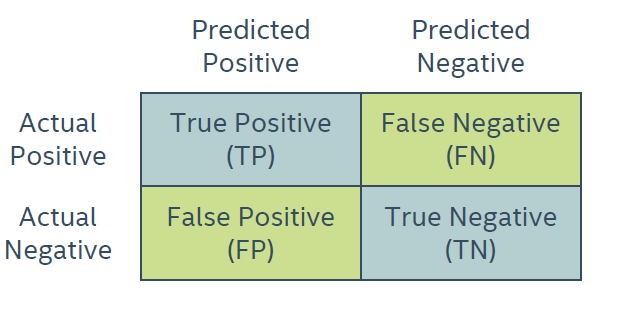
\includegraphics[width=0.5\linewidth]{confusion.PNG}
    \caption{Confusion matrix}
    \label{fig:my_label}
\end{figure}

\begin{itemize}
    \item Type I error - False Positive, Type II error - False Negative
    \item accuracy: $\frac{TP +TN}{TP +FN +FP +TN}$
    \item recall (sensitivity): $\frac{TP}{TP+FN}$
    \item precision: $\frac{TP}{TP+FP}$
    \item specifity: $\frac{TN}{FP+TN}$
    \item $F1 = 2 \frac{precision*recall}{precision + recall}$
    
\end{itemize}

Using these metrics the model can be evaluated using the Receiver Operating Characteristic (ROC):

\begin{figure}[H]
    \centering
    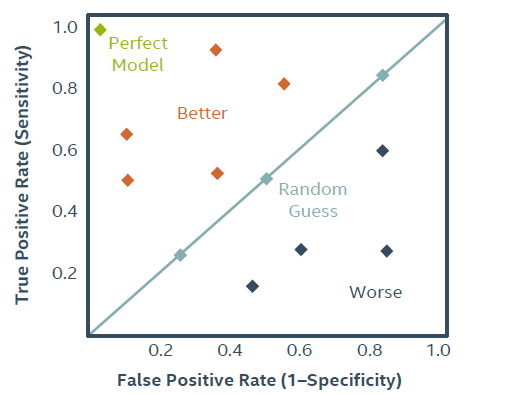
\includegraphics[width=0.5\linewidth]{roc.PNG}
    \caption{ROC}
    \label{fig:my_label}
\end{figure}

The curve is plotted by computing the ratio at different threshold levels (decision lines). A more efficient way of evaluating the precision of the model is to plot the Area Under Curve (AUC) graph.

\begin{figure}[H]
    \centering
    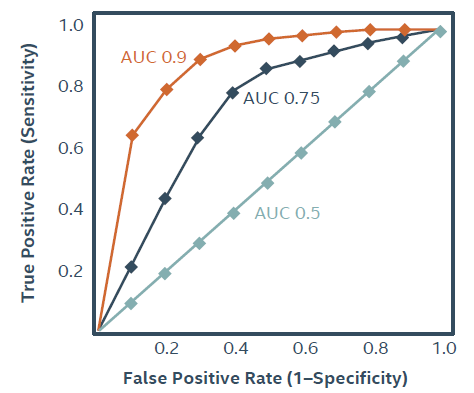
\includegraphics[width=0.5\linewidth]{auc.PNG}
    \caption{AUC}
    \label{fig:my_label}
\end{figure}

The AUC graph is based on a test of the probability that the model ranks a random positive example higher than a random negative example. One can also use the Precision Recall Curve (PR Curve) to determine the trade-off between precision and recall:

\begin{figure}[H]
    \centering
    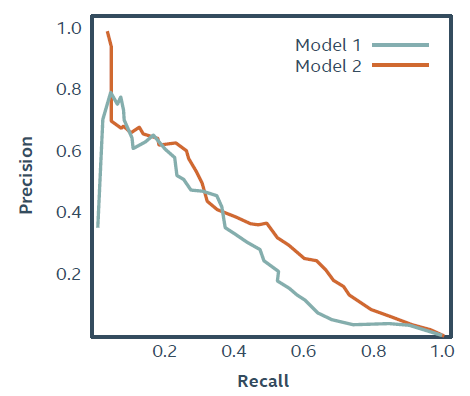
\includegraphics[width=0.5\linewidth]{pr.PNG}
    \caption{PR Curve}
    \label{fig:my_label}
\end{figure}

\subsection{Multiple class error metrics}

Most multi-class error metrics are similar to binary versions - they just require expanding as sums. E.g. accuracy for a 3-class problem is defined as:

\begin{equation}
    Accuracy=\frac{TP1+TP2+TP3}{Total}
\end{equation}

based on the following confusion matrix:

\begin{figure}[H]
    \centering
    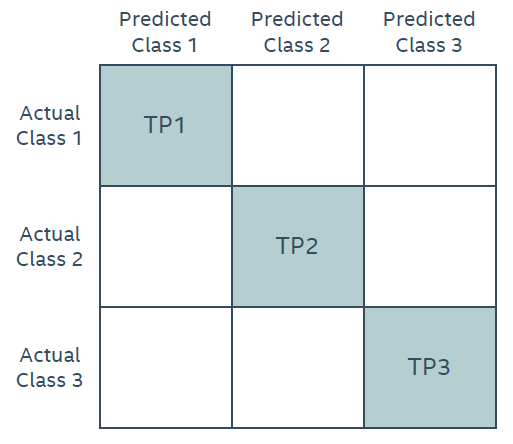
\includegraphics[width=0.5\linewidth]{confusion3.PNG}
    \caption{Confusion matrix for 3 class problem}
    \label{fig:my_label}
\end{figure}

\section{Naive Bayes}

\begin{figure}[H]
    \centering
    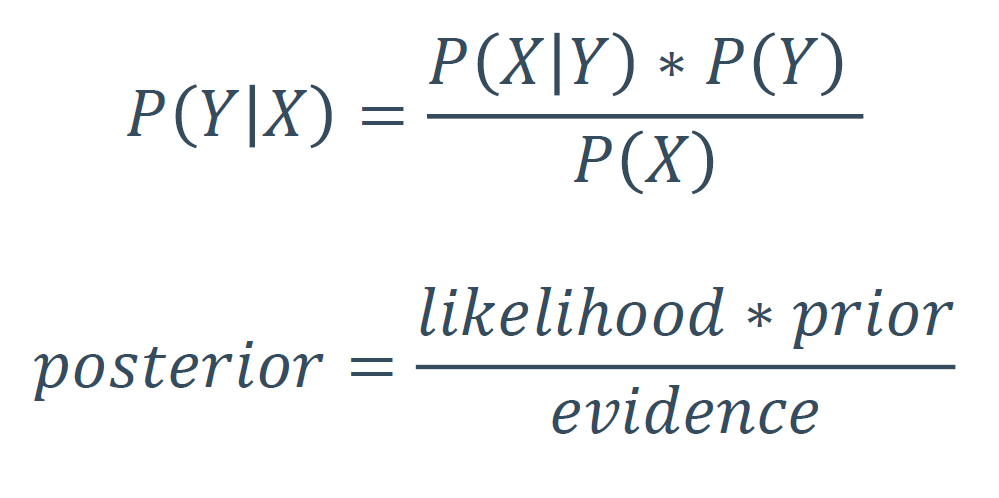
\includegraphics[width=0.5\linewidth]{bayes.PNG}
    \caption{Bayes theorem}
    \label{fig:my_label}
\end{figure}

Naive Bayes classification neglects evidence since don't want a normalized score, only the right class:

\begin{equation}
    P(X|Y)=P(X|Y) P(Y)
\end{equation}

For a classification problem X denotes the class and Y - features. Calculating the joint probabilities by expanding therefore a naive assumption that features are independent of each other is made. Classification is performed by computing the probability for each class and choosing the class with the highest score.

\subsection{Potential problems}

To prevent underflows caused by multiplication, one might take advantage of the "log trick" - multiply logs of each element of the equation to obtain the probabilities. 

Another potential problem is a zero probability of a class given a particular feature. A solution to this issue is to employ Laplace smoothing for categorical features:

\begin{equation}
    P(Y|X) = \frac{\lambda}{N + K\lambda}
\end{equation}

where N denotes the number of classes and K the number of unique options of a feature. $\lambda$ is usually set to unity.

\section{Support Vector Machines}

There is a similarity between SVMs and logistical regression - their objective is to draw a decision boundary. In case of SVMs this is performed by maximizing the separation region. The interpretation of the $\beta_i$ coefficients is a vector which is orthogonal to the hyperplane.

\begin{figure}[H]
    \centering
    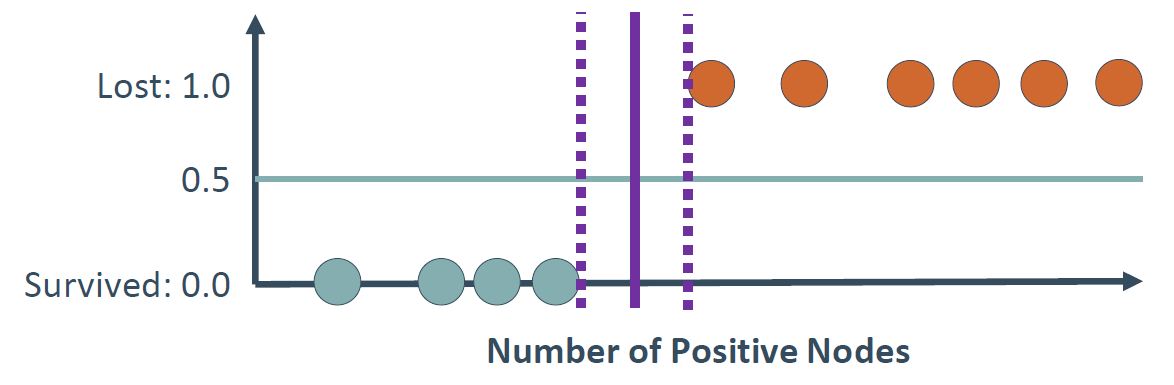
\includegraphics[width=\linewidth]{svm_plot.PNG}
    \caption{SVM - decision boundary}
    \label{}
\end{figure}

\begin{figure}[H]
    \centering
    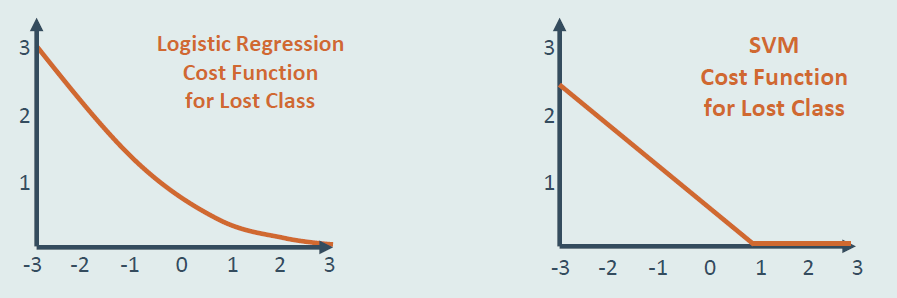
\includegraphics[width=\linewidth]{svmvslr.PNG}
    \caption{Comparison of cost functions - logistic regression and SVM}
    \label{fig:my_label}
\end{figure}

SVMs are sensitive to outliers:

\begin{figure}[H]
    \centering
    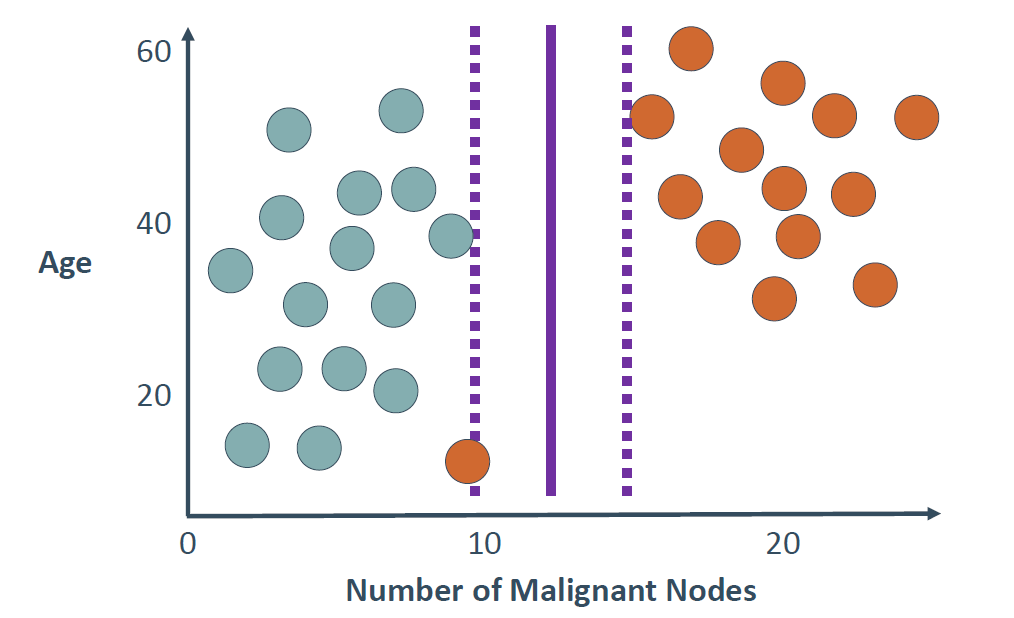
\includegraphics[width=0.5\linewidth]{svm_sens.PNG}
    \caption{SVM - outlier sensitivity}
    \label{fig:my_label}
\end{figure}

This problem can be overcome by regularization

\begin{equation}
    J(\beta_i) = SVMCost(\beta_i) + \frac{1}{C}\sum_i\beta_i
\end{equation}

SVMs can be extended to non-linear decision boundaries by means of kernels e.g. higher order features (squares of features etc., product of two features). Another example is the SVM Gaussian kernel which applies a Gaussian function for arbitrarily chosen features (each of them). Effectively this method transforms the space to a different coordinate system. The  resulting function is called Radial Basis Function.

SVMs are slow to train when many features and datapoints are analyzed. A solution to this problem is to construct an approximate kernel map with Stochastic Gradient Descent using Nystroem (subsampling) or RBF sampler and then fit a linear classifier. 

\section{Decision trees}

\begin{itemize}
    \item suitable for categorical, ordinal and continuous data (regression trees)
    \item features are split into binary decision - splitting ends when a) only one class remains, b) a maximum depth is reached, c) a performance metric is achieved
\end{itemize}

Greedy search - find a split which maximizes the information gained from the split. Several criteria can be chosen:

\begin{itemize}
    \item classification error equation: $E(t) = 1 - \underset{i}max[p(i|t)]$. The problem with this method is that since end nodes are non-homogenous (e.g. different number of observations), no further splits would occur (total information loss using this metric)
    \item entropy equation solves this problem: $H(t) = -\sum_{i=1}^n p(i|t)log_2[p(i|t)]$
    \item common choice - Gini index: $G(t)=1-\sum_{i=1}^n(p(i|t)^2$
\end{itemize}
\vline    
    
\subsection{Pros and cons}    
    
Decision trees are easy to interpret and implement using if/else logic, handle all data categories and don't require preprocessing or scaling.    
    
Potential problem with decision trees - overfitting. Small changes in data affect prediction greatly (high variance). The solution is to "prune" trees. Pruning can be based on the classification error threshold method.

\section{Bagging - bootstrap aggregation}

As previously mentioned, decision trees tend to overfit. A method of overcoming this issue is to create multiple trees, each using a subset of the data (approx. 2/3 of the data in one, sampling with replacement). The error of the individual tree measured on remaining data is called the "out-of-bag" error. However, fitting a bagged model doesn't produce coefficients like in e.g. logistic regression, but feature importances are estimated using oob error. Randomly permuting data for a particular feature affects the accuracy and this factor should be measured. Bagging performance increase with more trees (max improvement at approx. >50 trees).

\subsection{Strengths}
\begin{itemize}
    \item less variability than decision trees
    \item trees can be grown in parallel
\end{itemize}

\section{Random forest}

Although bagging reduces variances, the subsets of data are still corellated. To further de-correlate trees one might use subsets of features - $sqrt{m}$ for classification problems and $\frac{m}{3}$ for regression problems. This is called a random forest. 

For further randomness one can choose features and create splits randomly instead of choosing greedily - extra random trees (isolated random forest???).

\section{Boosting and stacking}
\subsection{Boosting}
The basic principle of boosting is to create consecutive classifiers by measuring residuals on the current classifier one and using them to create a decision stump on the following on. 

\begin{figure}[H]
    \centering
    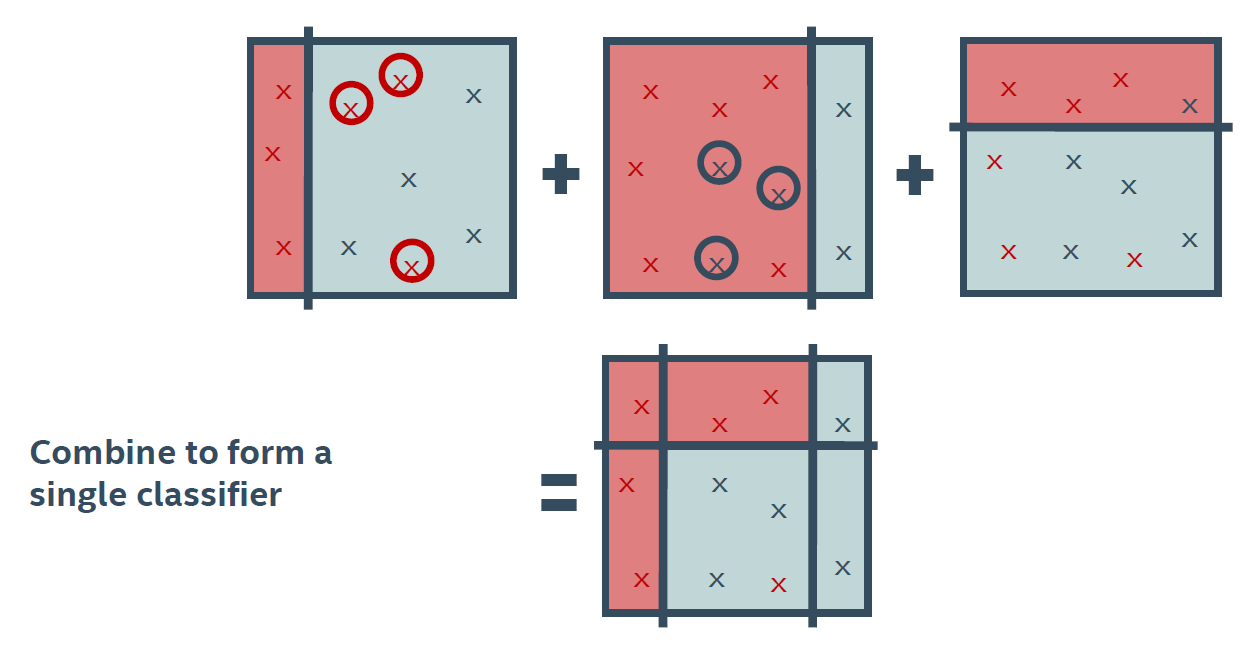
\includegraphics[width=0.5\linewidth]{boost1.PNG}
    \caption{Boosting - creating consecutive classifiers}
    \label{fig:my_label}
\end{figure}


The classifiers are then combined using a learning rate $\lambda$. 

\begin{figure}[H]
    \centering
    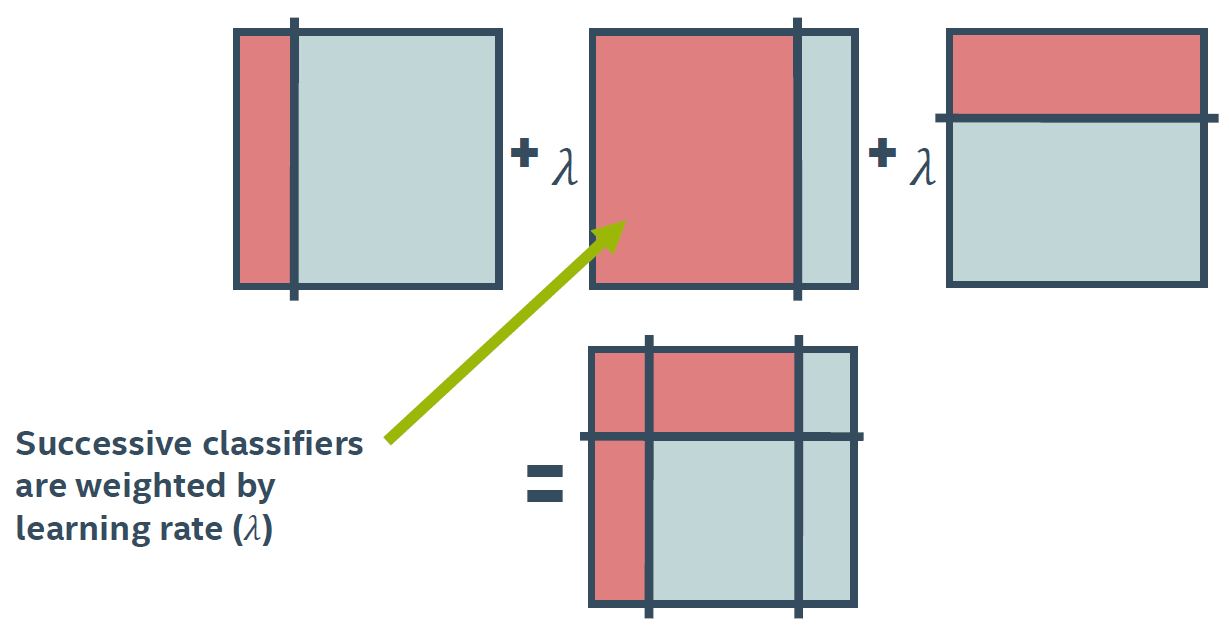
\includegraphics[width=0.5\linewidth]{boost2.PNG}
    \caption{Boosting - combining classifiers}
    \label{fig:my_label}
\end{figure}

The learning rate should be $< 1$ to prevent overfitting (form of regularization). Boosting utilizes different loss functions. The margin is determined for each point at each stage.  Value of loss function is calculated from margin.

\begin{figure}[H]
    \centering
    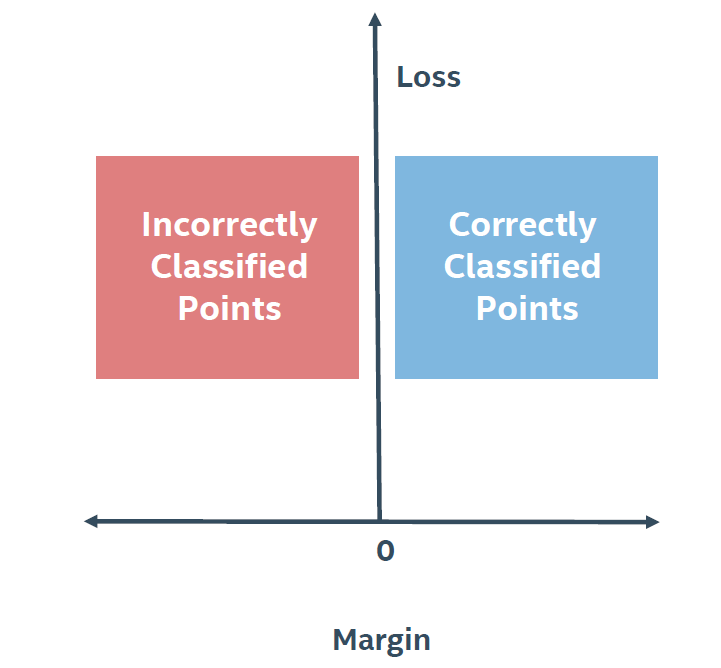
\includegraphics[width=0.5\linewidth]{boost3.PNG}
    \caption{Boosting - Loss function}
    \label{fig:my_label}
\end{figure}

There are several loss functions:
\begin{itemize}
    \item 0-1 loss function - "ideal" but difficult to optimize
    \item AdaBoost (Adaptive Boosting) - exponential loss function: $loss = e^{-margin}$, sensitive to outliers
    \item Gradient Boosting which uses different loss functions - common: binomial log likelihood loss function (deviance): $log(1+e^{-margin})$, more robust to outliers
\end{itemize}

\begin{figure}[H]
    \centering
    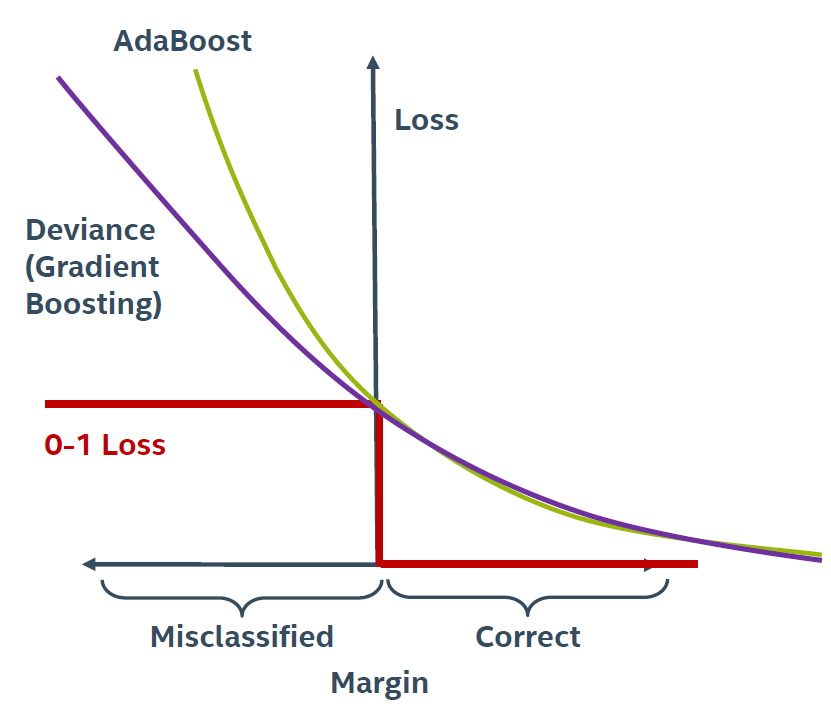
\includegraphics[width=0.5\linewidth]{boost4.PNG}
    \caption{Boosting - other loss functions}
    \label{fig:my_label}
\end{figure}

Boosting is performed for entire datasets, base trees are created succesively. Problem: easily overfits (shown below), cross-validation must be used to set number of trees.

\begin{figure}[H]
    \centering
    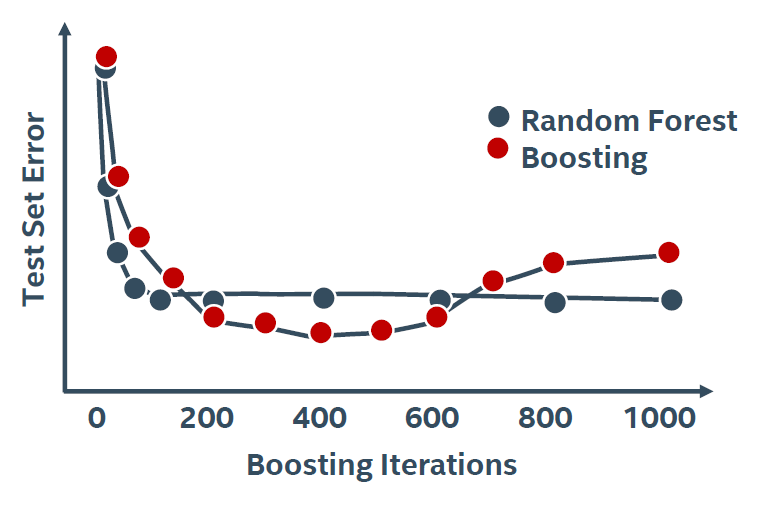
\includegraphics[width=0.5\linewidth]{boost5.PNG}
    \caption{Boosting - overfitting}
    \label{fig:my_label}
\end{figure}

\begin{figure}[H]
    \centering
    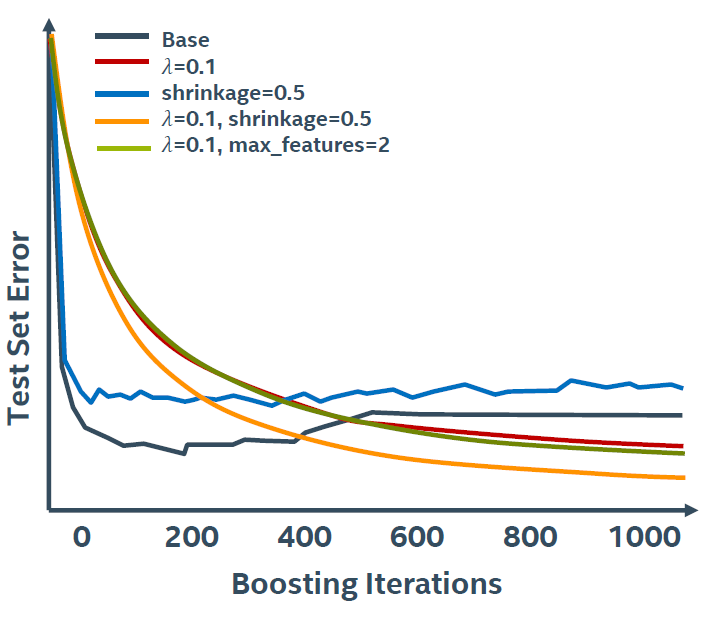
\includegraphics[width=0.5\linewidth]{boost6.PNG}
    \caption{Boosting - tuning the model}
    \label{fig:my_label}
\end{figure}

\subsection{Stacking}

Stacking is combining heterogenous classifiers as shown below:

\begin{figure}[H]
    \centering
    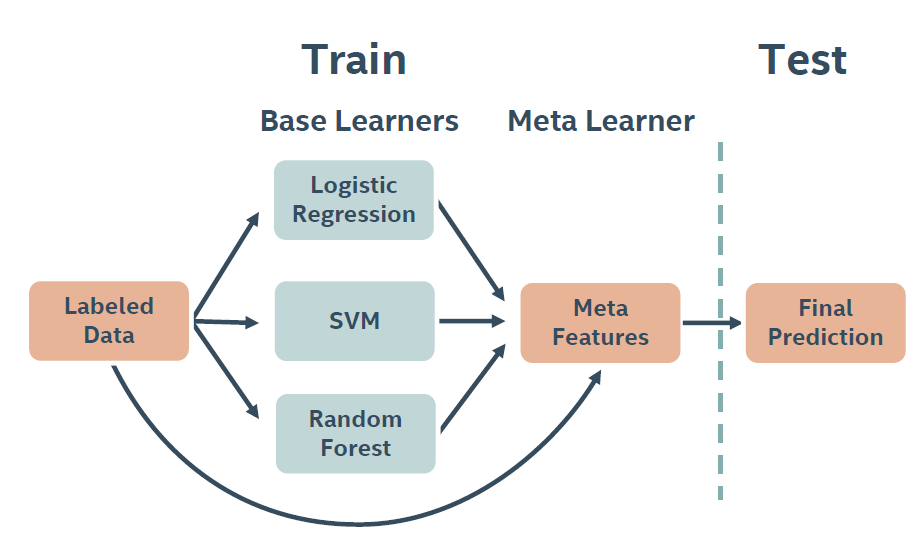
\includegraphics[width=0.5\linewidth]{stack.PNG}
    \caption{Stacking}
    \label{fig:my_label}
\end{figure}

Some data must be reserved if meta learner has hyperparameters. 

\section{Clustering}

\begin{itemize}
    \item unsupervised learning - identifying unknown structure in data
    \item 
\end{itemize}

\subsection{K-means algorithm}

\begin{enumerate}
    \item assign $k$ random cluster centers
    \item assign datapoints to nearest cluster center, creating clusters
    \item move cluster centers to the mean value of the cluster
    \item algorithm converges when points stop changing clusters
\end{enumerate}

The end result depends on the initial placement of cluster centers. The metric for assesing the quality of the model is the sum of squared distances from each point to its cluster, also known as inertia. The model can be fitted several times to choose the best version based on the metric. 

\subsection{Distance metrics}

\begin{itemize}
    \item Euclidian distance (L2), standard but sensitive to the curse of dimensionality
    \item Manhattan distance (L1, city block distance)
    \item Cosine distance: $cos(\theta)=\frac{A\cdot B}{||A||||B||}$, better or text data where location of occurence is less relevant
    \item Jaccard distance - applies to sets (word occurence): $1-\frac{A \cap B}{A \cup B}$
\end{itemize}

\subsection{Hierarchical Agglomerative Clustering algorithm}

\begin{enumerate}
    \item find the pair of closest points, merge
    \item find the next pair of closest points and merge
    \item if closest pair is two clusters, merge them into a larger cluster 
    \item stop when desired number of clusters is achieved or minimum average cluster distance reaches a set value
\end{enumerate}

Other linkage (stop criterium) methods are possible, e.g. complete linkage - max pairwise distance between cluster and all other points or average linkage - average pairwise distance between clusters and all other points. Merging of clusters can be performed using Ward linkage - based on best inertia. 

Other types of clustering:
\begin{itemize}
    \item mini-batch k-means
    \item affinity propagation
    \item mean shift
    \item spectral clustering
    \item ward clustering
    \item DBSCAN
\end{itemize}

\section{Dimensionality reduction}

The number of training examples required grows exponentially with dimensionality. Dimensionality is reduced by choosing subsets of features, omitting those which don't provide additional information - those which are correlated with other features. In example, when two features correlate we can create a new feature as a combination of both (Principal Component Analysis). 

\subsection{Single Value Decomposition}

Matrix factorization method used for PCA. PCA and SVD seek to find the vectors that capture the most variance, however they are sensitive to axis scale, so data has to be scaled. Transformation performed by PCA/SVD are linear. Although the method can be used for non-linear data, dimensionality reduction can fail. Similarly as in SVM, kernels can resolve problems with non-linear data.

\subsection{Multi-dimensional scaling}

\begin{itemize}
    \item non-linear transformation
    \item doesn't focus on maintaining overall variance, but geometric distance between points
    \item used for highf dimension data, NLP, image-based datasets
\end{itemize}

\chapter{Deep Learning basics}

\section{Neural Networks}

\begin{itemize}

\item computation engine built from layers containing activation functions - each node of a layer is a function with inputs from the previous layer; layers do not have to be linearly stacked;

\item each neuron is a unit of regression - larger networks are needed because one neuron only permits a linear decision boundary;

\item input layer, hidden layers, output layers;

\item net input - sum of weighted inputs which is fed to the activation function, activations - outputs of activation functions;

\item epoch - single pass through all of the training data;

\end{itemize}•

\section{Training neural nets}

Training is employed by computing an output, comparing the output to the correct results, computing the loss function and then apply backpropagation - adjusting weights. Calculating the gradient for neural nets is achieved using the chain rule. First, derivatives of the loss function with respect to every weight in the network are computed. The activation functions tend to have handy derivatives, e.g. the sigmoid function $f(z) = \frac{1}{1 + e^{-z}}$ has the following derivative: $f'(z) = f(z)(1-f(z))$. According to the chain rule, the loss function derivatives are computed sequentially layer by layer, starting from the last one. 

\begin{figure}[H]
    \centering
    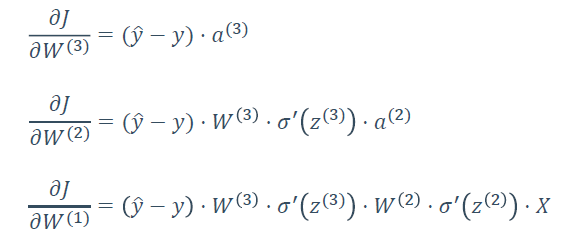
\includegraphics[width=0.5\linewidth]{chain_rule.PNG}
    \caption{Chain rule - each term can be interpreted as an estimate of the change of activations with respect to the input, backpropagation is employed by multiplication of terms from the following layers.}
    \label{fig:my_label}
\end{figure}

The problem with the sigmoid function is that the gradients become very small for early layers ("vanishing gradient" problem).  

\subsection{Other activation functions}

\begin{itemize}
\item hyperbolic tangent function $tanh(z) = \frac{sinh(z)}{cosh(z)} = \frac{e^{2x}-1}{e^{2x} + 1}$
\item rectified linear unit (RELU)

\begin{figure}[H]
    \centering
    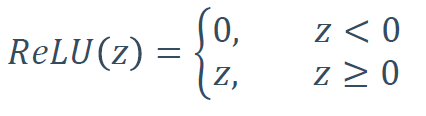
\includegraphics[width=0.5\linewidth]{relu.PNG}

\end{figure}

\item leaky rectified linear unit 

\begin{figure}[H]
    \centering
    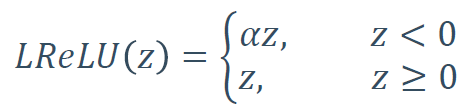
\includegraphics[width=0.5\linewidth]{lrelu.PNG}

\end{figure}


\end{itemize}

\subsection{Updating weights }

In the classic approach, derivates are obtained for the entire dataset, however this requires a considerable computational effort, so the algorithm becomes slow for large datasets. Stochastic gradient descent can be a remedy to this problem - the steps are less informed but their number is higher and the introduced noise should be balanced out over time. When using SGD, a smaller step size is needed, and data regularization usually helps. Alternatively, one can choose a compromise approach - mini-batch GD (batches of 16-32 data points).

\begin{figure}[H]
    \centering
    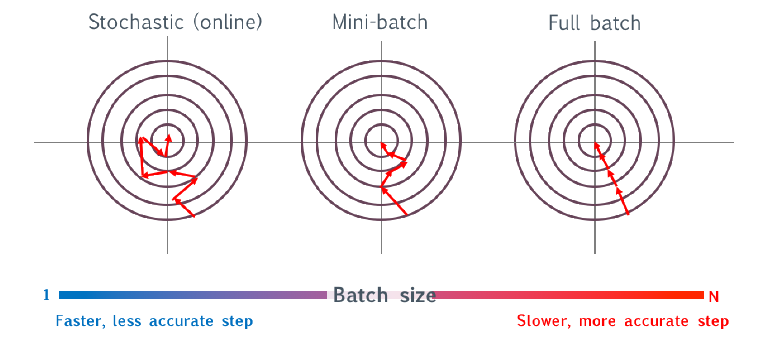
\includegraphics[width=0.75\linewidth]{NNGD.PNG}

\end{figure}

In full batch GD, one step per epoch. In SGD / Online, n steps per epoch (n = training set size). In minibatch - n / batch size. A metric for learning is the number of epochs. To avoid cyclical movement effects, it is recommended to shuffle the data after each epoch - this ensures that the chosen batches are random.  

The inputs should be scaled to the $[-1, 1]$ or $[0, 1]$ interval. Furthermore, one can standarize (make the variable approximately std. normal) the inputs:

\begin{equation}
x_{i} = \frac{x_i - \hat{x}}{\sigma}
\end{equation}

\begin{equation}
\sigma = \sqrt{ \frac{1}{n} \sum_{i=1}^{n} (x_i - \hat{x})^2}
\end{equation}



\subsection{Classification problems with neural nets}

\begin{itemize}
\item for binary classification, the final layers has a single node and a sigmoid activation funtion; output between 0 and 1 and can be interpreted as probability; handy derivative; analogous to logistic regression;
\item for multiclass classification the final layer is a vector with the length equal to the number of classes, utilizes the \textit{softmax} sigmoid extension to multiclass problems: $softmax(z_{i} = \frac{e^{z}_{i}}{\sum_{k=1}^{K} e^{Z}_k})$. Categorical cross entropy is used as the loss function: $C.E. = - \sum_{i=1}^{n} y_{i} log(\hat{y_{i}})$

\end{itemize}

\subsection{Regularization techniques for deep learning}

In order to regularize - prevent overfitting - the following measures can be taken:

\begin{itemize}
\item regularization penalty in the cost function - e.g. explicitly adding a penalty to the loss function for having high weights (similar to Ridge Regression):
\begin{equation}
J = \frac{1}{2n} \sum_{i=1}^{n} (\hat{y_i} - y_i)^2 + \lambda \sum_{j=1}^{m} W_i^2
\end{equation}

\item dropout - a technique where at each training iteration (batch) we randomly remove a subset of neurons; makes the network more robust because it doesn't rely on individual pathways; at test time, the weight is rescaled based on the time it was active;
\item early stopping - choosing rules as to when the training is stopped, e.g. check log-loss function every 10 epochs to determine whether the model hasn't started to overfit;
\item stochastic / mini batch GD also help to some degree

\end{itemize}



\subsection{Optimizers}

Optimizers are tools for determining the update of weights. The standard formula $W :=  W - \alpha \nabla  J$ often provides unsatisfactory performance. Momentum optimizers smooths out the variation of standard updates, changing weights a little bit at every update. E.g. Nesterov momentum:

\begin{equation}
\nu_t = \eta \nu_{t-1} - \alpha \nabla (J - \eta \nu_{t-1})
\end{equation}

\begin{equation}
W := W - \eta_t
\end{equation}

where $\eta$ is the momentum. The idea is that overshooting is controlled by looking "ahead". A different approach si the AdaGad optimizer. The idea is to scale the update separately for each weight. Sum of previous updates is kept and new updates are divided by factor of the previous sum.

\begin{equation}
W := W - \frac{\eta}{\sqrt{G_t} + \epsilon} \odot \nabla J
\end{equation}

A popular method nowadays is the RMSPROP which is similar to AdaGrad. However, rather than using the sum of previous gradients, older ones are decayed more than recent ones. Therefore, it is more adaptive to recent updates. Another popular method - ADAM - uses both 1st and 2nd order change information and decayover time.


\section{Convolutional Neural Networks - CNNs}

So far the structure of input data was not constrained - inputs were treated interchangeably. However, not all data-driven problems, are free of relationships between data points. Images are an example of such data - they are characterized by the following traits:

\begin{enumerate}
\item pixels have a topology
\item lighting and contrast
\item human visual system
\item nearby pixels tend to have similar values - the role of gradients
\item edges and shapes
\item translation and scale invariance

\end{enumerate}

If images were treated in the same way as regular data, that is if each pixel had its own weights, the number of weights would be tremendous and so would be the variance. We have to introduce a bias to look for patterns. 

\subsection{In a nutshell}

\begin{itemize}
\item built up from kernels - grids of weights overlaid on an image, centered on one pixel; used for traditional imahe processing techniques: bluring, sharpen, edhe detection, emboss;

\begin{figure}[H]
    \centering
    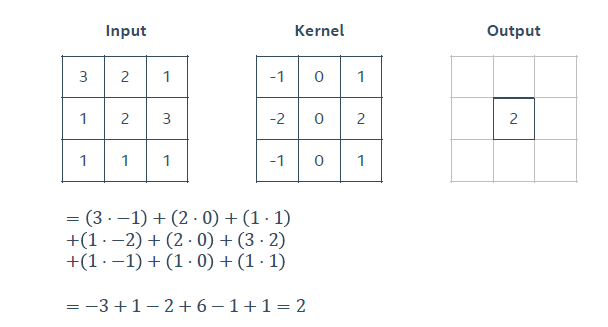
\includegraphics[width=0.75\linewidth]{kernel_example.PNG}
    \caption{Kernel example}
\end{figure}

\end{itemize}

The neural network learns which kernels are most useful, uses them over the entire image (translation invariance). Effectively, the number of parameters is reduced whereas variance is mitigated. The dimensions of a kernel are referred to as grid size, typically it is such that a central point can be distinguished. As a consequence of this kind of discretization of an image, the network suffers from an edge effect as a center pixel cannot be determined for corners. This issue is resolved by padding - adding 0 value (typically) pixels around the frame of the image.

\subsection{Convolution settings}

\begin{itemize}
\item stride - the step size between neighbouring kernels, if greater than 1 than the output dimension is reduced;
\item depth - number of kernels used for learning, often the number of channels describing a pixel, RGB -3, CMYK-4;
\end{itemize}

Beyond increasing the stride, another way of reducing the problem size is pooling - mapping a patch of pixels to a single value. There are several methods for choosing a numeric value to represent a patch - e.g. maximum value (max-pool), average of values (average-pool).

\subsection{Convolution structure}

\begin{figure}[H]
    \centering
    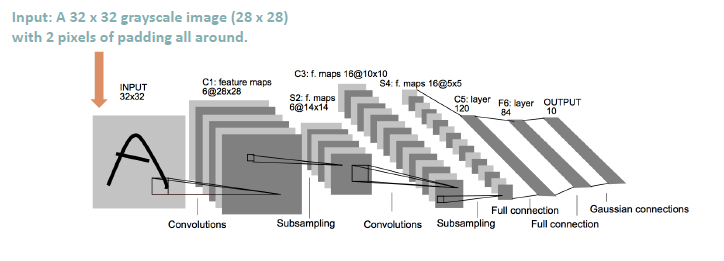
\includegraphics[width=1\linewidth]{lenet.PNG}
    \caption{Le-Net 5 CNN architecture}
\end{figure}

\begin{enumerate}
\item input;
\item convolutional layer, depth=6 (six different kernels used for learning), making the output $28x28x6$;
\item pooling layer with stride 2;
\item convolutional layer on downsized data, depth is increased to 16;
\item another pooling layer;
\item then the kernels are flattened to a vector whose size is reduced by a series of fully connected layers;
\item softmax output with size equal to number of classes;
\end{enumerate}

\subsection{Training convolutional neural networks}

\begin{enumerate}
\item the first layers are the hardest (i.e. slowest) to train due to the vanishing gradient issue; at the same time, they are responsible for capturing primitive features which are quite general, not case specific;

\item later layers capture features which are more specific to a particular classification problem, they are easier to train since adjusting their weights has a more immediate impact on the final result;

\end{enumerate}



\section{Transfer learning}

There are several difficulties associated with training a model from scratch:
\begin{itemize}
\item  very large datasets;
\item many training iterations;
\item computational cost;
\item time for hyper-parameter optimization.

\end{itemize}

However, general features captured by early layers should generalize and the weights can be easily stored. Transfer learning is employed by using the early layers of a pre-trained network, re-training the later layers for a specific application. Additional training of a pre-trained network on a new dataset is referred to as fine-tuning. 

\subsection{Guidelines for fine-tuning}

\begin{enumerate}
\item The higher the similarity of the data and problem definition between the new case and the original one, the less fine-tuning is necessary. 

\item The more data is available for the new problem, the more benefit is taken from longer and deeper fine-tuning.

\item The new data cannot differ substantially in form with respect to the data that the model was trained on. 

\end{enumerate}



\end{document}